\subsection{Aplicaci\'on a la bah\'ia de Concepci\'on}

A partir de informaci\'on  de cartas n\'auticas del Servicio Hidrogr\'afico y Oce\'anico de la Armada de Chile [CITAS] se interpol\'o la topograf\'ia y batimetr\'ia correspondiente a la zona de la bah\'ia de Concepci\'on, y se utiliz\'o el software computacional AnuGA[CITA] para generar la malla de elementos triangulares en el lugar de inter\'es, como se puede ver en la figura \ref{fig:bati-talcahuano}. La malla posee un total de 2697 nodos y 57600 tri\'angulos, y se impuso que el \'area de cada triangulo fuera menor que $57600m^2$. 

La condici\'on de borde por el lado que da hacia el oc\'eano no es trivial de implementar, y como una primera aproximaci\'on se simul\'o como un borde s\'olido, lo cual es consistente con el caso l\'imite en que las ondas quedan completamente atrapadas al interior. De esta forma, la bah\'ia completa se consider\'o como si estuviera cerrada por todos los bordes. 

Dadas estas definiciones, los seis primeros modos de oscilaci\'on y los per\'iodos asociados se encuentran representados en la figura \ref{fig:modos_talcahuano}.



\begin{figure}
  \centering
  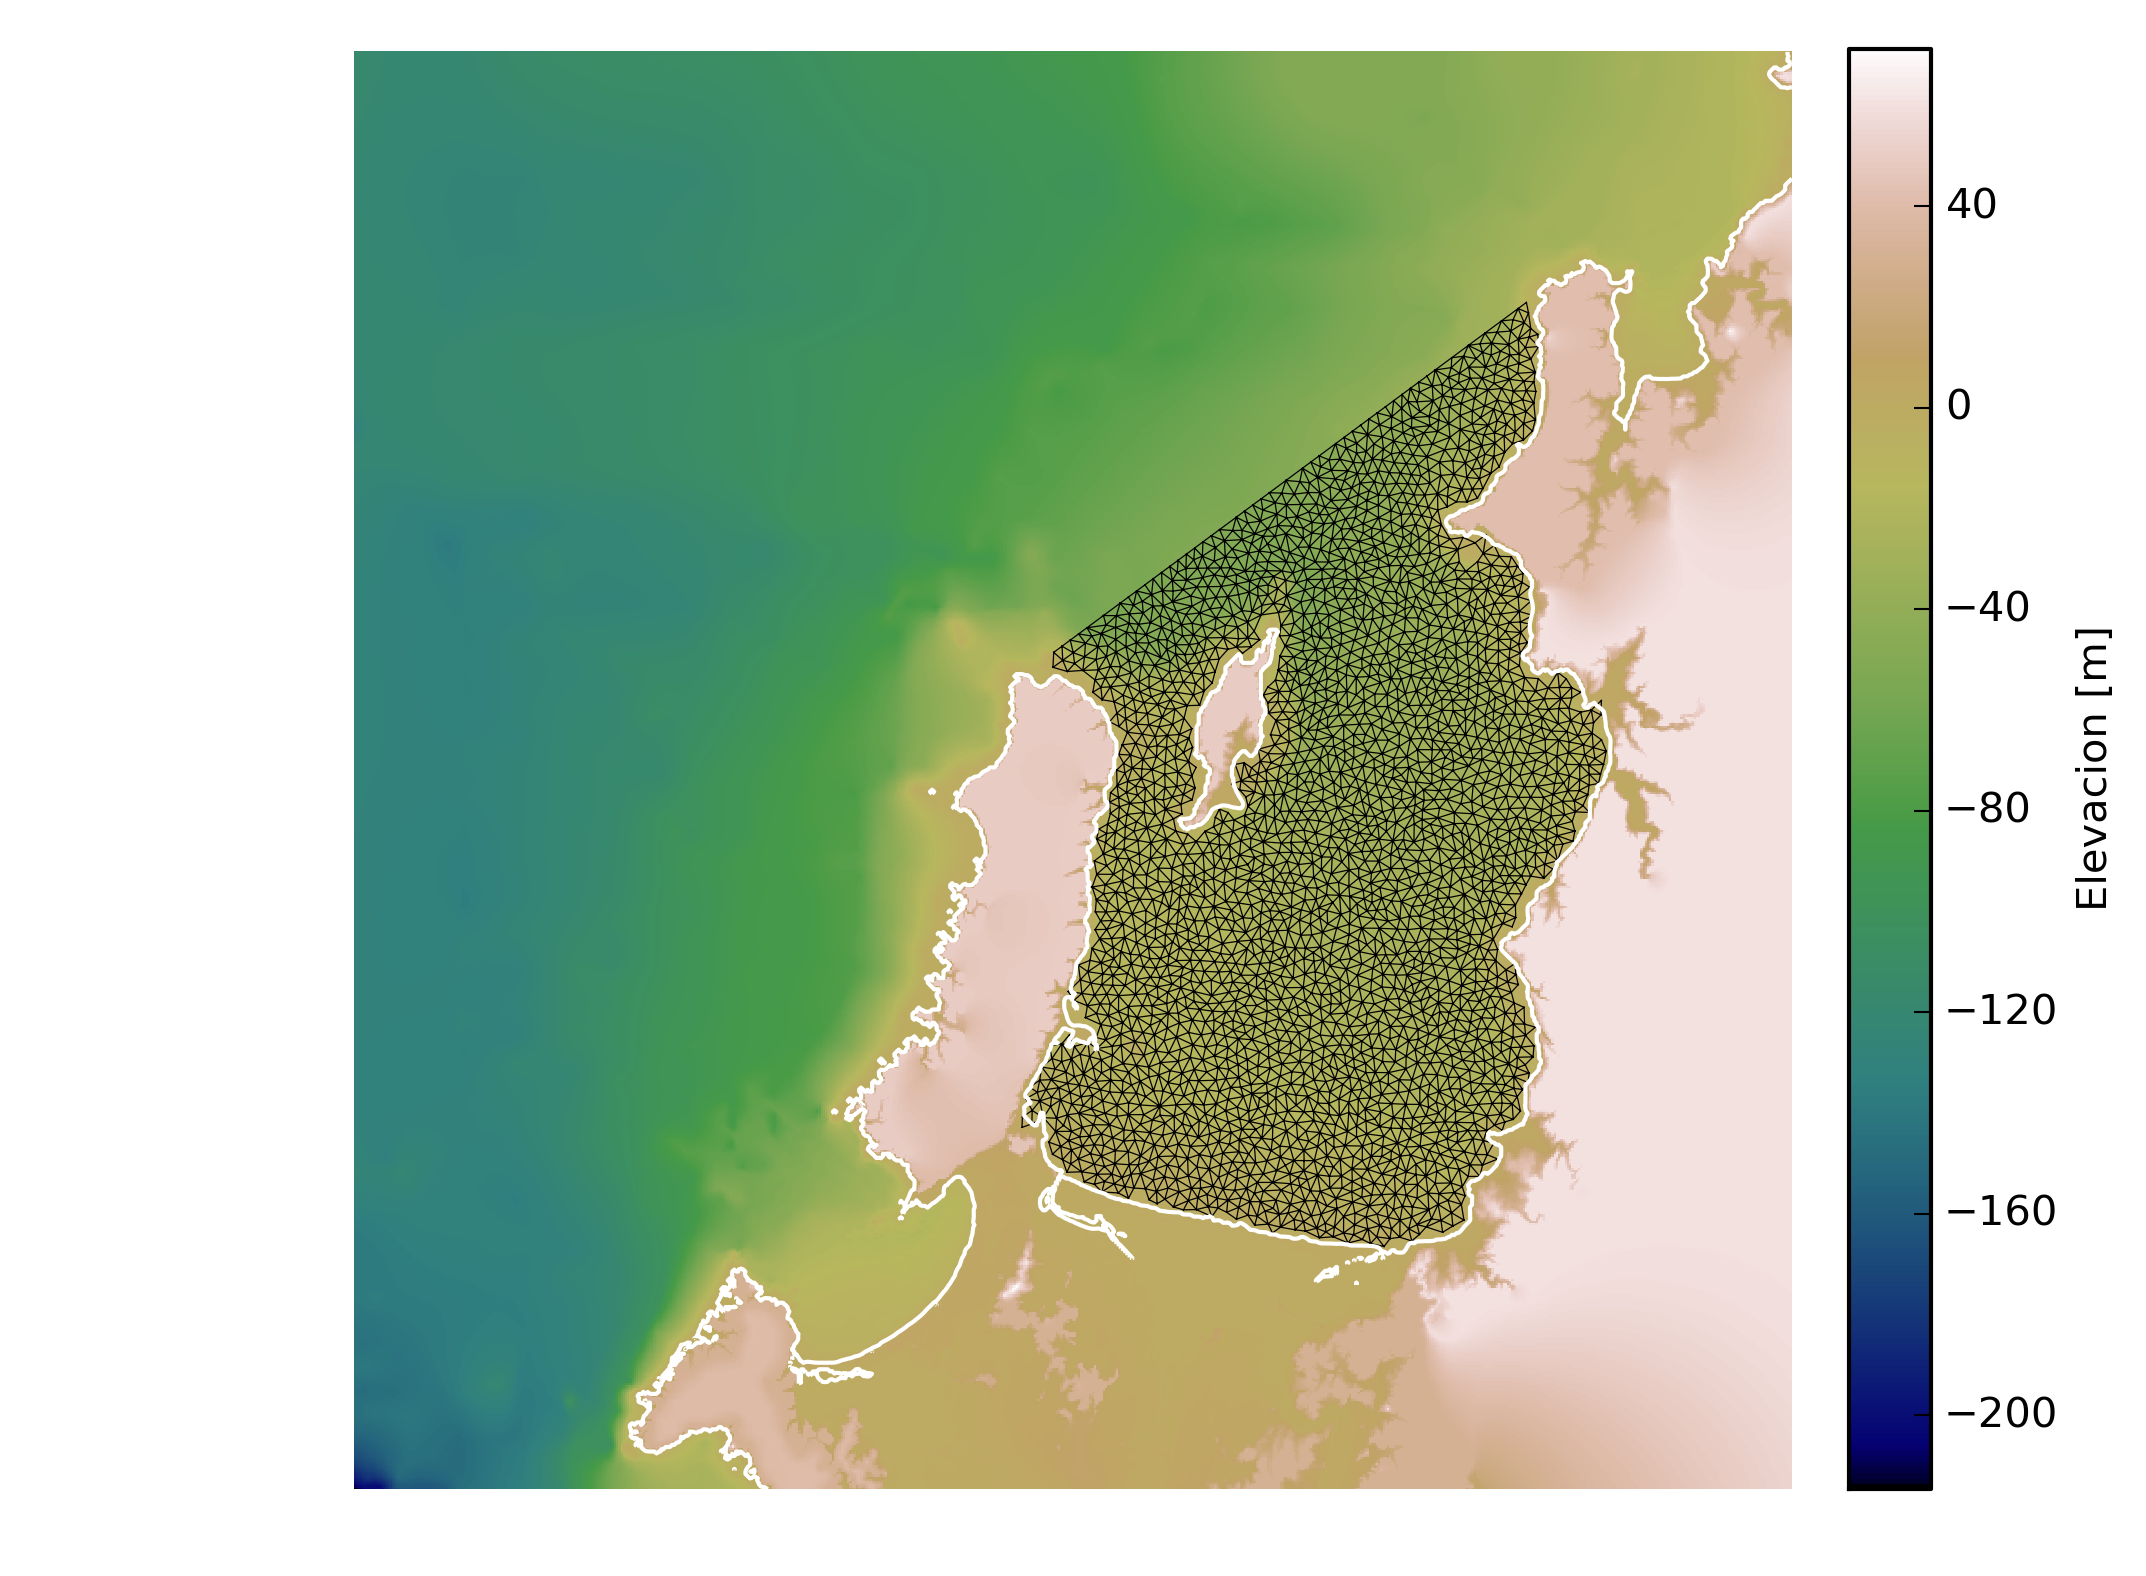
\includegraphics[width=15cm]{figuras/04bati+malla.png}
  \caption{ Batimetr\'ia y topograf\'ia de Talcahuano y malla triangular utilizada en la bah\'ia de Concepci\'on}  
  \label{fig:bati-talcahuano}
\end{figure}

\begin{figure}
  \begin{subfigure}{0.5\textwidth}
    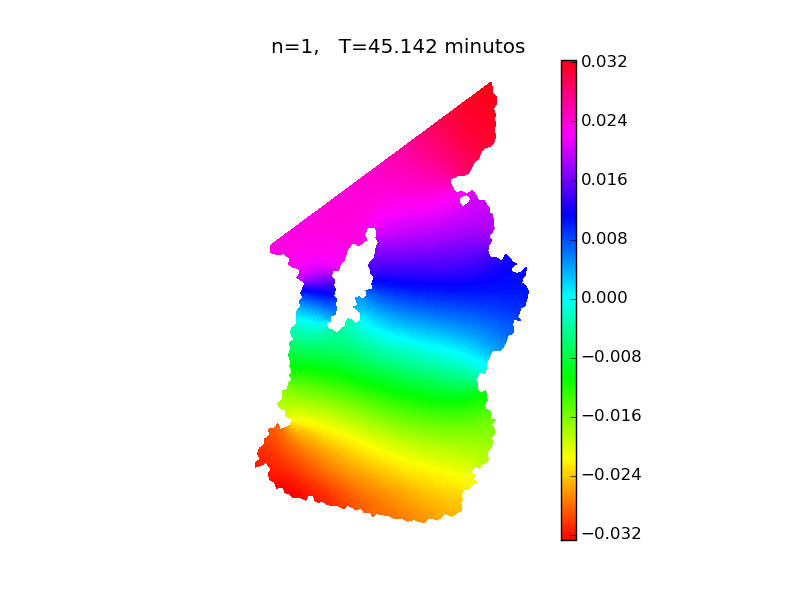
\includegraphics[width=\textwidth]{figuras/modos1.png}
  \end{subfigure}
  ~
  \begin{subfigure}{0.5\textwidth}
    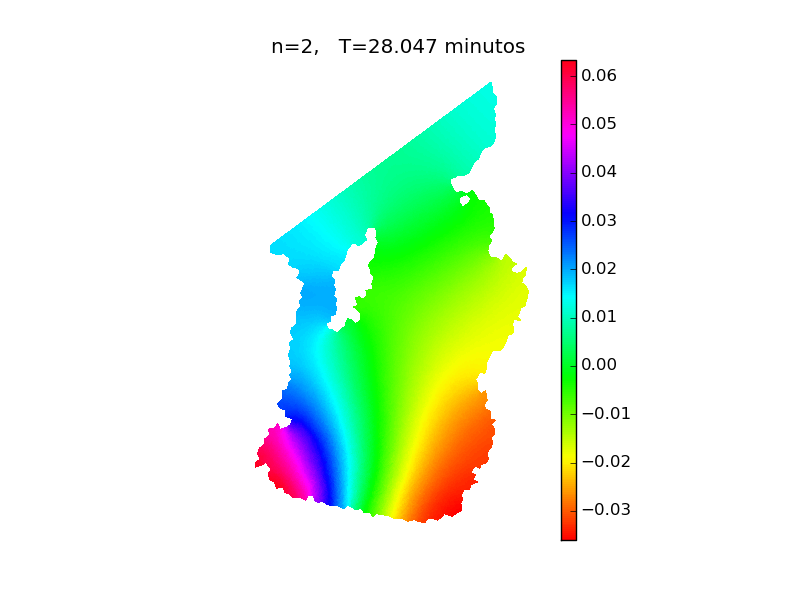
\includegraphics[width=\textwidth]{figuras/modos2.png}
  \end{subfigure}
  ~
  \begin{subfigure}{0.5\textwidth}
    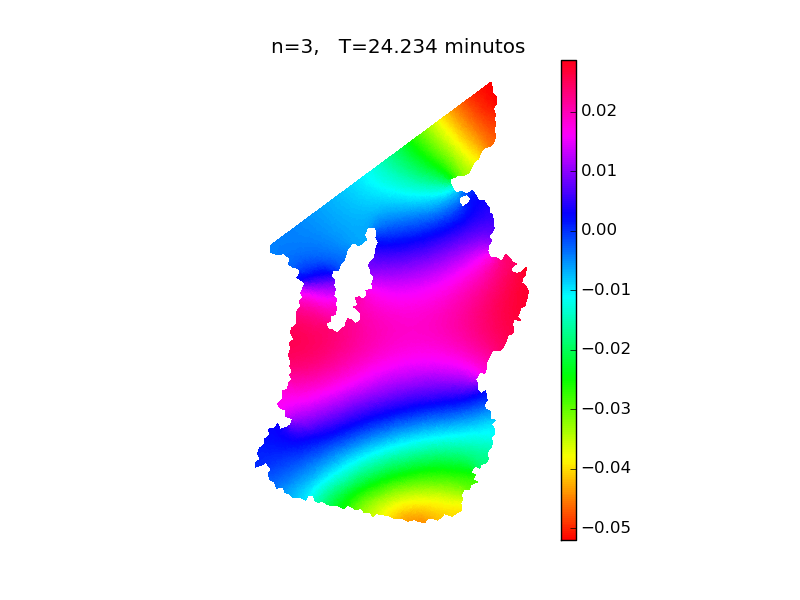
\includegraphics[width=\textwidth]{figuras/modos3.png}
  \end{subfigure}
  ~
  \begin{subfigure}{0.5\textwidth}
    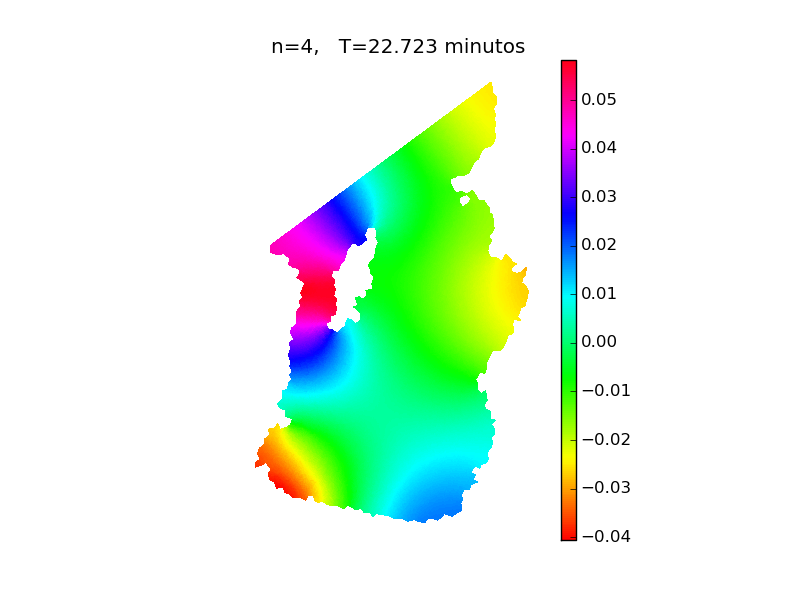
\includegraphics[width=\textwidth]{figuras/modos4.png}
  \end{subfigure}
  \\
  \begin{subfigure}{0.5\textwidth}
    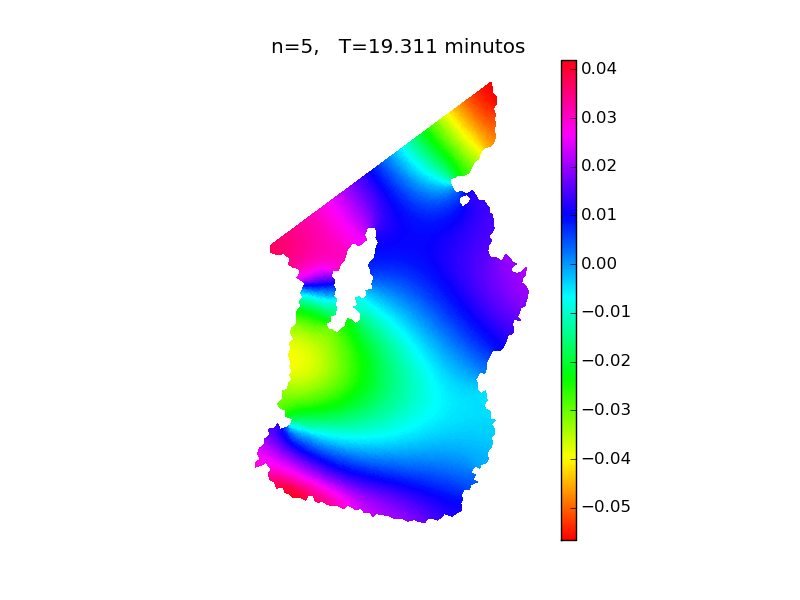
\includegraphics[width=\textwidth]{figuras/modos5.png}
  \end{subfigure}
  ~
  \begin{subfigure}{0.5\textwidth}
    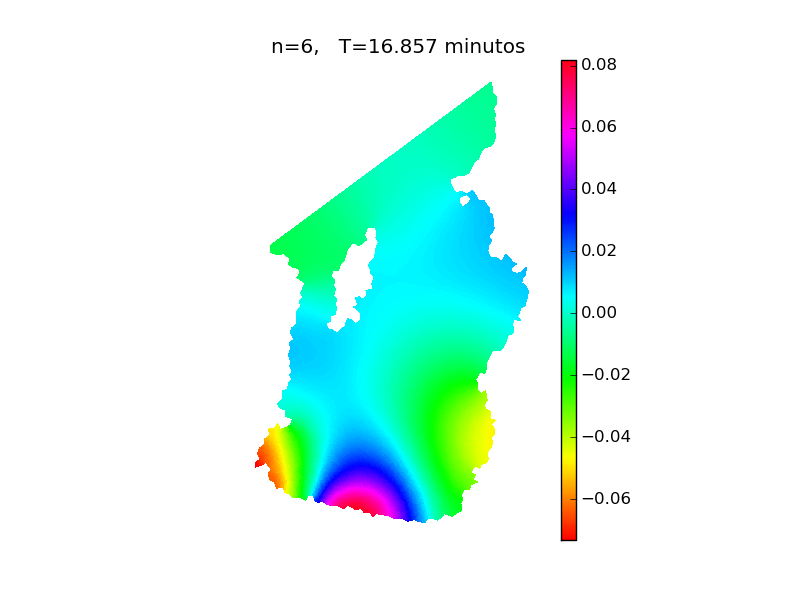
\includegraphics[width=\textwidth]{figuras/modos6.png}
  \end{subfigure}
  
  \caption{Primeros seis modos y per\'iodos de oscilaci\'on obtenidos para la configuraci\'on de la bah\'ia de Concepci\'on}
  \label{fig:modos_talcahuano}
\end{figure}